% 原书 p.168–p.171（PDF p.176–p.179）
\section{辛容量（Symplectic Capacity）}

% >>> p176
描述／确定一个区域的大小，其源头是 Gromov 非压缩定理（定理 1.5.1）：在那里，区域
之间的辛嵌入对区域的参数是敏感的。本节中，我们将集中于系统研究 $\C^n$ 中区域大小
的一种方式。记 $\mathcal{LD}^{2n}$ 为 $\C^n$ 中全体刘维尔区域之集。下面我们引入
$\mathcal{LD}^{2n}$ 上一类重要的辛不变量。

\begin{keytakeaways}
\begin{itemize}
  \item 几何图像：辛容量是赋予刘维尔区域一个「辛大小」的函数，它满足单调性、
        共形齐次性与球—圆柱归一化三条公理；体积不满足归一化，故不是辛容量。
  \item 数学工具：辛容量的存在性等价于 Gromov 非压缩定理；由辛同调构造的
        $c_{\mathrm{SH}}$（式 (6.25)）给出 Gromov 定理的一行证明。
  \item 关键结论：Gromov 宽度 $w_G$ 是一切辛容量中最小的一个（练习 6.4.1）；
        Viterbo 猜想断言凸区域上所有球归一化容量相等，从而给出等周型不等式
        (6.26)。
  \item 前沿视角：ECH 容量（例 6.4.2）与 McDuff 定理（定理 6.4.1）把四维辛嵌入
        问题完全转化为数列 $N(a,b)_k$ 的比较。
\end{itemize}
\end{keytakeaways}

\begin{wdefn}{6.4.1（见 [124] 第 2.1 节）}
  \textbf{辛容量}（symplectic capacity）是一个函数
  $c\colon\mathcal{LD}^{2n}\to\R_{\ge0}\cup\{\infty\}$，它满足下述公理。
  \begin{enumerate}[label=(c\arabic*)]
    \item 对 $U,V\in\mathcal{LD}^{2n}$，若 $U$ 辛嵌入到 $V$ 中，则 $c(U)\le c(V)$。
    \item 对任意 $\lambda>0$ 与 $U\in\mathcal{LD}^{2n}$，$c(\lambda U)=\lambda c(U)$，
          其中 $\lambda U:=\{\sqrt{\lambda}\cdot x\mid x\in U\}$。
    \item 对 (1.13) 中定义的辛球 $B^{2n}(1)$ 与辛圆柱
          $Z^{2n}(1)=B^2(1)\times\R^{2n-2}$，有 $c(B^{2n}(1))=c(Z^{2n}(1))=1$。
  \end{enumerate}
  公理 (c3) 称为\textbf{球归一化}（ball-normalization）条件。
\end{wdefn}

\begin{wrem}{6.4.1}
  (i) $\C^n$ 中的体积\emph{不}是辛容量，因为它违反 (c3)。(ii) 在某些情形下，辛
  容量 $c\colon\mathcal{LD}^{2n}\to\R_{\ge0}\cup\{\infty\}$ 满足公理 (c1) 与 (c2)，
  但只满足 (c3) 的一个较弱版本：$c(B^{2n}(1))>0$ 且 $c(Z^{2n}(1))<\infty$。一个
  标准的例子是\textbf{拉格朗日容量}，通常记作 $c_{\mathrm{Lag}}$ 或 $c_L$。关于
  $c_{\mathrm{Lag}}(B^{2n}(1))$ 与 $c_{\mathrm{Lag}}(Z^{2n}(1))$ 的显式计算，见
  [53] 第 1.2 节。
\end{wrem}

当辛容量的概念被提出时，公众已经知道这样的函数总是存在的（尽管这一点完全不显然），
它来自下述结果。

\begin{wprop}{6.4.1}
  辛容量的存在性等价于 Gromov 非压缩定理。
\end{wprop}

\begin{wproof}
  假设存在定义 6.4.1 中的辛容量。则由其全部公理，若 $B^{2n}(r)$ 辛嵌入到
  $Z^{2n}(R)$ 中，则
  \[
    r=r\,c(B^{2n}(1))=c(B^{2n}(r))\le c(Z^{2n}(R))=R\,c(Z^{2n}(1))=R.
  \]
  反之，对任意 $U\in\mathcal{LD}^{2n}$，考虑下述量
  \begin{equation}\tag{6.24}
    w_G(U):=\sup\{r\ge0\mid
    \exists\ \text{辛嵌入}\ B^{2n}(r)\hookrightarrow U\}.
  \end{equation}
  显然 $w_G$ 满足公理 (c1)。公理 (c2) 可按下述方式验证：
  \begin{align*}
    w_G(\lambda U)
    &=\sup\{r\ge0\mid\exists\ \text{辛嵌入}\ B^{2n}(r)\hookrightarrow\lambda U\}\\
    &=\sup\left\{r\ge0\mid\exists\ \text{辛嵌入}\ 
      B^{2n}\left(\frac{r}{\sqrt{\lambda}}\right)\hookrightarrow U\right\}\\
    &=\sup\{\lambda r'\ge0\mid\exists\ \text{辛嵌入}\ 
      B^{2n}(r')\hookrightarrow U\}
      =\lambda w_G(U).
  \end{align*}
\end{wproof}

% >>> p177
最后，若假设定理 1.5.1 成立，则 $w_G$ 满足 (c3)。因此按定义 6.4.1，$w_G$ 是一个
辛容量。

在实践中，构造辛容量的途径众多——有些更接近动力学，另一些更接近代数或拓扑（很好的
综述见 [52]）。下述练习表明，在上述命题 6.4.1 的证明中构造的 $w_G$ 相当特殊。历史上，
$w_G$ 被称为\textbf{Gromov 宽度}（Gromov width）。

\begin{wexer}{6.4.1}
  证明：任意辛容量 $c$ 都满足 $c\ge w_G$，其意义是对任意
  $U\in\mathcal{LD}^{2n}$ 有 $c(U)\ge w_G(U)$。换言之，在所有辛容量之中，Gromov
  宽度 $w_G$ 是最小的一个。那么是否存在最大的辛容量？
\end{wexer}

基于 6.3 节详述的辛同调理论，我们也可以构造自己的辛容量。

\begin{wexam}{6.4.1}
  固定刘维尔区域 $W\in\mathcal{LD}^{2n}$，并假设它已经是非退化的（定义见例 6.3.1
  正上方的那一段）。则我们可以按下述步骤定义函数 $c_{\mathrm{SH}}(W)$，如下方的
  交换图所示。\hfill$//$
\end{wexam}

\begin{figure}[htbp]
  \centering
  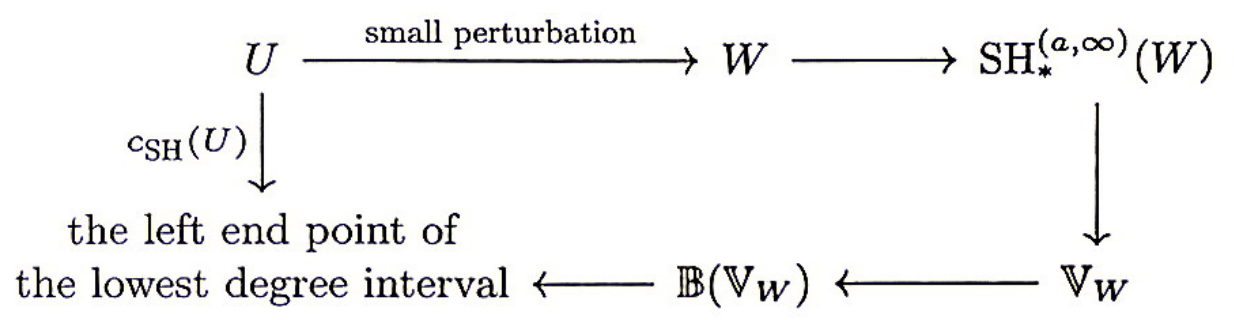
\includegraphics[width=0.85\linewidth]{figures/fig_p177_1.png}
  \caption*{例 6.4.1 的交换图：$U$ 经小扰动得到 $W$，再取过滤辛同调；$W$ 的持续模
    $\mathbb{V}_W$ 的条形码 $\mathbb{B}(\mathbb{V}_W)$ 的最低次数区间的最左端点，
    即 $c_{\mathrm{SH}}(U)$（原书 p.169 示意图，无编号；PDF p.177）}
\end{figure}

具体说来，应用定义 6.3.1 中的过滤辛同调并把它们组装，得到持续 $\Z_2$-模
$\mathbb{V}_W$。于是我们的函数定义为
\begin{equation}\tag{6.25}
  \ln c_{\mathrm{SH}}(W)=
  \text{条形码 }\mathbb{B}(\mathbb{V}_W)\text{ 中最低次数区间的最左端点},
\end{equation}
它称为 $W$ 的\textbf{辛同调容量}（symplectic homology capacity）。

若 $W$ 不是非退化的，则可在 $\mathcal{LD}^{2n}$ 中任取一列在 $C^0$-拓扑下收敛到
$W$ 的非退化刘维尔区域 $\{W_i\}_{i\in\N}$；一个稳定性结果（见 [211] 中的定理 1.8）
蕴含 $c_{\mathrm{SH}}(W)$ 是良定义的，即为标量列
$\{c_{\mathrm{SH}}(W_i)\}_{i\in\N}$ 的极限。

可以证明 $c_{\mathrm{SH}}$ 确实是 $\mathcal{LD}^{2n}$ 上的辛容量。例如，为验证公理
(c3)，例 6.3.5 中的计算结果可助一臂之力。由 (6.25) 的定义与适当的逼近，我们有
\[
  c_{\mathrm{SH}}\bigl(B^{2n}(1)\bigr)=e^{\ln1}=1.
\]
再用辛椭球 $E(1,N,\cdots,N)$（$N\notin\Q$，$N\to\infty$）逼近辛圆柱
$Z^{2n}(1)$。于是
\[
  c_{\mathrm{SH}}\bigl(Z^{2n}(1)\bigr)
  =\lim_{N\to\infty}c_{\mathrm{SH}}\bigl(E(1,N,\cdots,N)\bigr)=e^{\ln1}=1.
\]

% [Tutor Note: 原文疑误——(6.25) 与例 6.4.1 的交换图都称，$\ln c_{\mathrm{SH}}(W)$
% 取「最低次数区间的最左端点」。但按例 6.3.5，$E(1,\pi)$ 在最低次数处的条形码为
% $\{(-\infty,0]\}$，其最左端点是 $-\infty$，这与随后的
% $c_{\mathrm{SH}}(B^{2n}(1))=e^{\ln1}=1$ 矛盾：要得到 $e^{\ln1}$，只能取该区间的
% 有限端点（即右端点）$0$。可能的解释是原书把条形码的过滤参数轴画反了（或约定
% 「最左」指 $r$ 轴上的较大一侧）。此处按原文直译，未作改动；已记入
% review_ch06.md，建议核对原文。]$，
% 其最左端点为 $-\infty$？注意这里「最左端点」应理解为该区间在过滤参数 $r$ 下的
% 右端点 $\ln1=0$（条形码条 $(-\infty,0]$ 的「最左」在通常绘制中指向右端），
% 故 $c_{\mathrm{SH}}=e^0=1$。这个约定上的细节使 (6.25) 的文字表述略有歧义；
% 阅读时应以例 6.3.5 与 $e^{\ln1}=1$ 的计算为准。]

% >>> p178
有趣的是，公理 (c1) 与 (c2) 实际上更难，因为其中涉及 $\mathrm{SH}$ 的函子性质
（见 [182] 第 9.5 节）。

作为 $c_{\mathrm{SH}}$ 的一个直接应用，下面给出 Gromov 非压缩定理的一行证明。

\begin{wproof}[定理 1.5.1 的证明]
  例 6.4.1 表明，通过 (6.25) 定义的 $c_{\mathrm{SH}}$ 是一个辛容量，于是由命题
  6.4.1 即得所需结论。
\end{wproof}

人们或许会问：不同的辛容量之间能相差多少？这应与区域的几何形状密切相关。例如，若
$W\in\mathcal{LD}^{2n}$ 局部具有某个「细颈」，而那里存在一条非常短的闭 Reeb 轨道
$\gamma$，则 $c_{\mathrm{SH}}(W)$ 可能非常小（因为由 $\gamma$ 给出的闭哈密顿轨道的
作用量很小，见 (6.25) 的定义）。然而 $w_G(W)$ 仍可能很大。这是一个典型的「区域
不够圆」的例子（示意图见图 6.14）。辛几何中下述著名猜想给出了相反方向的结论。

\begin{figure}[htbp]
  \centering
  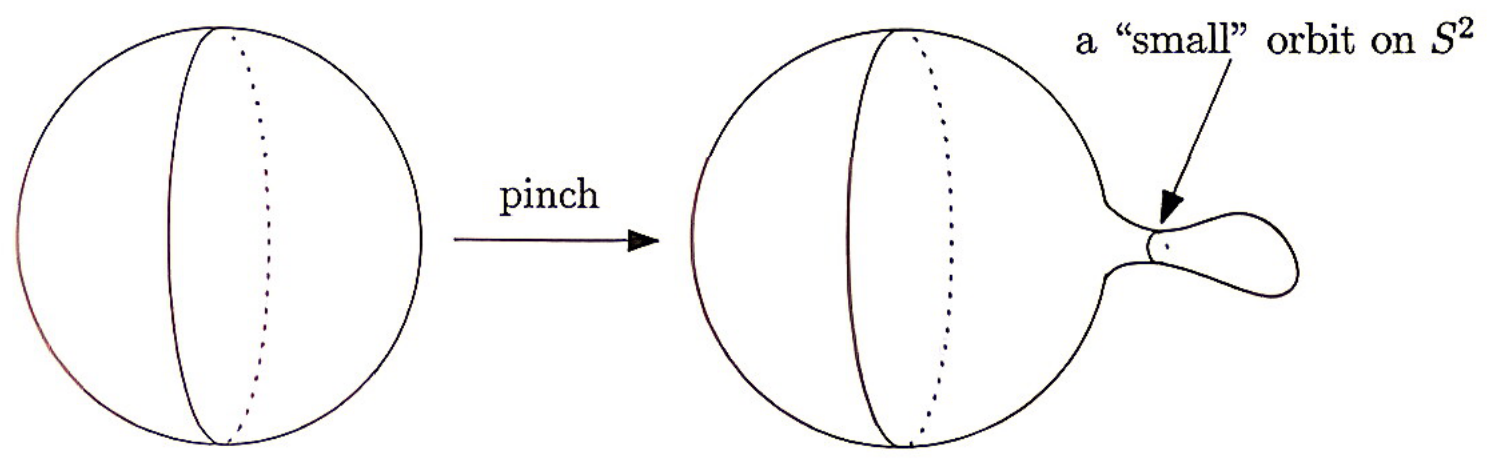
\includegraphics[width=0.85\linewidth]{figures/fig_p178_1.png}
  \caption*{图 6.14\quad $S^2$ 上的小「收缩」（原书 p.170, Figure 6.14；PDF p.178）}
\end{figure}

\begin{wconj}{6.4.1（Viterbo [235]）}
  在 $\R^{2n}$ 的任意给定凸区域上，所有球归一化辛容量都重合。
\end{wconj}

假设该猜想成立，便得到下述等周型结果：对 $\R^{2n}$ 的任意凸区域 $U$，以及定义 6.4.1
中的任意球归一化辛容量 $c$，有
\begin{equation}\tag{6.26}
  c(U)\le\bigl(n!\,\Vol_{\R^{2n}}(U)\bigr)^{\frac{1}{n}}.
\end{equation}
此外，对任意 $r>0$，取 $U=B^{2n}(r)$ 可使等号成立。确实，假设猜想 6.4.1 成立，则对
任意凸区域 $U\subset\R^{2n}$，存在 $r>0$ 使得 $c(U)=w_G(U)=r$。由 (6.24) 中 $w_G$
的定义，存在辛嵌入 $B^{2n}(r)\hookrightarrow U$。于是，由于辛同胚保持体积，体积比较
给出
\[
  \frac{r^n}{n!}=\Vol_{\R^{2n}}\bigl(B^{2n}(r)\bigr)\le\Vol_{\R^{2n}}(U).
\]
这就给出所需不等式。把 (6.26) 换一种说法：在所有体积
$\Vol_{\R^{2n}}(U)$ 固定的凸区域 $U$ 之中，辛容量最大的是球 $B^{2n}(r)$。

% [Tutor Note: 含糊点拨——(6.26) 的推导依赖两个事实：(i) 猜想 6.4.1 把任意球归一化
% 容量与 $w_G$ 等同；(ii) $w_G$ 的定义给出辛嵌入 $B^{2n}(r)\hookrightarrow U$，再由
% 体积单调性得 $r^n/n!\le\Vol(U)$。注意这里用到 $\Vol(B^{2n}(r))=r^n/n!$（在
% $\omega_{\mathrm{std}}$ 下），而 $n!$ 因子正是等周不等式的「辛修正」——它与
% Gromov 宽度、以及 Viterbo 容量在凸区域上的共同值同源。当 $U$ 非凸时 (6.26) 一般
% 不再成立（例如细颈区域）。]

% >>> p179
猜想 6.4.1 已在许多情形下得到证实（见 [109, 21, 134, 189]）。有趣的是，最近在四维
情形，Ostrover--Haim--Kislev 的工作 [110] 构造了该猜想的一个相当初等的反例。与此同时，
Abbondandolo--Editmar--Kang 的工作 [3] 证明：在 $\R^4$ 的凸区域上，在所有现存辛容量
之中至多有两个容量，一个是 $w_G$，其余全部重合。

% [Tutor Note: 原文疑误——[3] 的作者姓名原文印作「Abbondandolo-Editmar-Kang」，
% 其中「Editmar」很可能是「Edtmair」（O.~Edtmair）的排印错误；此处译文保留原文
% 写法以免改动文献，已在 review_ch06.md 中记录，建议核对 [3] 原文。]

回忆注 6.4.1 的 (ii)：定义 6.4.1 中的公理 (c3) 是可以放松的。一个直接推论是：可以
构造一列辛容量 $c_1\le c_2\le\cdots$，其中只有第一个 $c_1$ 满足球归一化条件。这类
容量序列的一个著名例子是 \textbf{ECH 容量}（其中「ECH」代表嵌入切触同调，embedded
contact homology），由 M.~Hutchings 在 [127] 中发明。这些容量只适用于四维情形；而
适用于更高维情形的类似容量序列由 Gutt--Hutchings 在 [108] 中构造。

\begin{wexam}{6.4.2（Proposition 1.2 in [127]）}
  四维辛椭球 $E(a,b)$ 的 ECH 容量由下式算出：
  \[
    c_k^{\mathrm{ECH}}\bigl(E(a,b)\bigr):=N(a,b)_k,
    \qquad k\ge0,
  \]
  其中 $N(a,b)$ 是 $a,b$ 的一切非负整数线性组合（计重数）按递增方式排成的序列，
  而 $N(a,b)_k$ 是它的第 $k$ 个元素。\hfill$//$
\end{wexam}

特别地，$c_*^{\mathrm{ECH}}$ 可用于给出辛椭球之间辛嵌入的障碍。事实上，得益于 D.
McDuff 的下述结果，从不同的 $E(a,b)$ 读出的序列 $N(a,b)$ 的单调性，也给出它们之间
辛嵌入的存在性。

\begin{wthm}{6.4.1（[152] 中的定理 1.1）}
  对任意四维辛椭球 $E(a,b)$ 与 $E(c,d)$，$E(a,b)$ 辛嵌入到 $E(c,d)$ 中当且仅当对
  任意 $k\ge0$ 有 $N(a,b)_k\le N(c,d)_k$。
\end{wthm}

\begin{wexer}{6.4.2（Conjecture 1.12 in [127], Theorem 1.1 in [61]）}
  计算极限
  \[
    \lim_{k\to\infty}
    \frac{c_k^{\mathrm{ECH}}\bigl(E(a,b)\bigr)^2}{k},
  \]
  并用几何方式解释这一结果。
\end{wexer}

对任意给定的 $k\ge0$，显式写出全部 $N(a,b)_k$ 几乎是不可能的；而有效的估计或计算
公式可见 [115] 中的命题 A.1。迄今为止，$c_*^{\mathrm{ECH}}(E(a,b))$ 是处理四维辛
嵌入问题最有用的辛容量之一。

% [Tutor Note: 术语/记号依据——「ECH 容量」中的 ECH 指 embedded contact homology
% （嵌入切触同调），由 Hutchings 基于 Taubes 的 ECH=SW 定理发展而来；$N(a,b)$ 的
% 定义（$a,b$ 的非负整数线性组合按重数递增排列）与椭球的 Reeb 轨道周期谱
% $\{ka+lb\}$ 一一对应，这正是 ECH 容量可从椭球显式算出的原因。四维之外，Gutt--
% Hutchings 用一个类似的「谱序列」构造了高维容量序列，故 (6.4.2) 一类结论目前
% 仍是四维辛嵌入理论的专属工具。]
